\documentclass[10pt]{article}
\usepackage[T2A]{fontenc}
\usepackage[utf8]{inputenc}
\usepackage[english,russian]{babel}
\usepackage{amsfonts, amssymb, amsmath, amsthm}
\usepackage{graphicx}
\usepackage{subcaption}
\usepackage[font=small]{caption}
\usepackage{wrapfig}
\usepackage{enumitem}
\setlist{noitemsep}
\usepackage[text={14cm, 20cm}]{geometry}

\graphicspath{{./resources/theory/}}

\renewcommand{\leq}{\leqslant}
\renewcommand{\geq}{\geqslant}
\renewcommand{\phi}{\varphi}
\newcommand{\R}{\mathbb{R}}
\newcommand{\E}{\mathbf{E}}
\renewcommand{\C}{\mathcal{C}}
\newcommand{\bF}{\bar{\mathcal{F}}}
\newcommand{\F}{\mathcal{F}}
\newcommand{\cY}{\check{Y}}
\newcommand{\wY}{\widetilde{Y}}
\newcommand{\wDelta}{\widetilde{\Delta}}
\renewcommand{\wp}{\widetilde{p}}
\newcommand{\wq}{\widetilde{q}}
\newcommand{\wf}{\widetilde{f}}
\newcommand{\wrho}{\widetilde{\rho}}
\newcommand{\hq}{\widehat{q}}
\newcommand{\eps}{\varepsilon}

\newtheorem{theorem}{Теорема}
%\newtheorem{lemma}{Лемма}
%\newtheorem{remark}{Замечание}

\title{Обучение без учителя. \\Разделение смеси распределений. \\Кластеризация.}
\author{Федяев~И., Понизова~В.}
\date{22.10.2019} % (optional)

\begin{document}
\maketitle

\section{Обучение без учителя}

Обучение без учителя (Unsupervised learning) --- раздел машинного обучения, в котором изучается класс задач обработки данных, в которых известны
только описания множества объектов (признаки объектов) из обучающей выборки, и требуется обнаружить внутренние зависимости, существующие
между объектами. В отличие от обучения с учителем, правильные <<ответы>> или <<метки>> для объектов не известны.


Задачи обучения без учителя можно разделить на следующие типы:
\begin{itemize}
\item Кластеризация
\item Поиск ассоциативных правил
\item Заполнение пропущенных значений
\item Сокращение размерности
\item Визуализация данных
\end{itemize}

\textbf{Задачи кластеризации.}
Выборка объектов разбивается на непересекающиеся подмножества, называемые кластерами, так, чтобы каждый кластер состоял из схожих объектов, 
а объекты разных кластеров существенно отличались.

\textbf{Задачи поиска правил ассоциации.}
Задача состоит в том, чтобы найти такие наборы признаков, и такие значения этих признаков, 
которые особенно часто (неслучайно часто) встречаются в признаковых описаниях объектов.

\textbf{Задача восполнения пропущенных данных.}
Значения некоторых признаков для некоторых объектов могут отсутствовать. Однако, некоторые методы обработки данных требуют на вход данные без пропусков.
Для заполнения отсутствующих значений часто применяют следующий подход. 
Считая данный признак целевым, строят алгоритм, прогнозирующий его значение в зависимости от других признаков. Пропущенные значения заполняют прогнозами. 
Эта операция проделывается со всеми признаками, имеющими пропущенные значения. 

\textbf{Задачи сокращения размерности.}
Исходная информация представляется в виде признаковых описаний, причём число признаков может быть достаточно большим. 
Задача состоит в том, чтобы представить эти данные в пространстве меньшей размерности, по возможности, минимизировав потери информации.

\textbf{Задачи визуализации данных.}
Некоторые методы кластеризации и снижения размерности строят представления выборки в пространстве размерности два. 
Это позволяет отображать многомерные данные в виде плоских графиков и анализировать их визуально, 
что способствует лучшему пониманию данных и самой сути решаемой задачи.

Основной темой данного конспекта является описание различных подходов к кластеризации.

\section{Кластеризация}
\subsection{Описание задачи}

Целью кластеризации является разделение данных на несколько непересекающихся кластеров. 
При этом, под кластеризацией можно понимать два типа задач: непосредственная кластеризация и сегментация.
Задачи первого типа можно описать следующим способом.
Пусть имеется подмножество $X \subset \R^n$, которое мы будем называть пространством объектов, 
и задана функция расстояния между объектами $\rho: X \times X \rightarrow [0, \infty)$.
Пусть имеется также некоторая конечная выборка объектов $X^m = \{x_1, \dots, x_m\} \in X$.

Необходимо найти множество кластеров $Y$ и алгоритм кластеризации $a: X \rightarrow Y$ такие, что:
	\begin{itemize}
		\item каждый кластер состоит из близких объектов (относительно $\rho$);
		\item объекты разных кластеров различались существенно.
	\end{itemize}

\begin{figure}[h]
	\centering
	\begin{subfigure}{0.4\textwidth}
		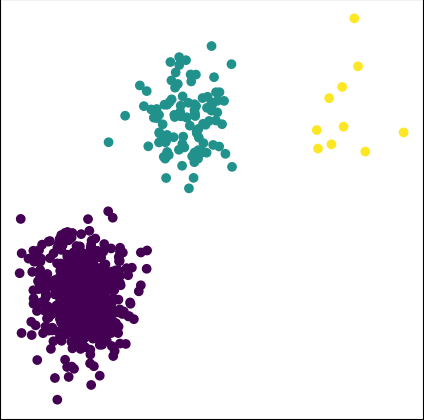
\includegraphics[scale=0.3]{Clusters.png}
		\caption{Пример кластеризации.}
		\label{fig:clusters}
	\end{subfigure}
\begin{subfigure}{0.4\textwidth}
		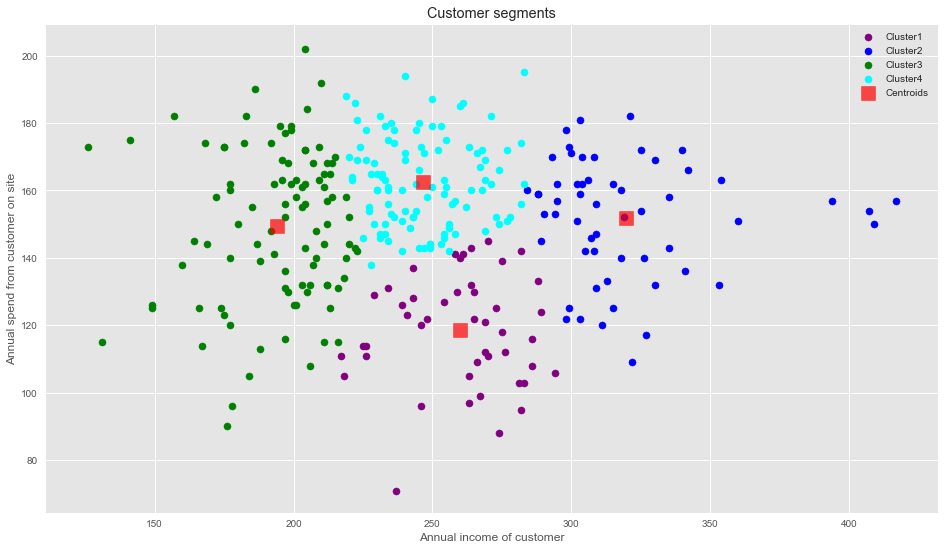
\includegraphics[scale=0.15]{cloud.png}
		\caption{Пример сегментации.}
		\label{fig:cloud}
	\end{subfigure}
	\caption{}
	\end{figure}

Приведённое выше описание фиксирует лишь общее намерение при кластеризации данных, и при этом не является точной математической постановкой задачи.

Идеальные данные для такого типа кластеризации выглядят примерно так, как представлено на рис.~\ref{fig:clusters}. 
В таких данных мы видим чётко отделённые друг от друга облака объектов. Кластеризация данных в таком случае производится с целью обнаружить неоднородность и
понять, стоит ли её интерпретировать как структуру в данных или продолжить анализ кластеров отдельно.

Для задач сегментации, условие на сильное различие объектов разных кластеров игнорируется. В таком случае облако объектов может выглядеть как один кластер, 
однако данные всё равно разделяются на большее число кластеров (см. рис.~\ref{fig:cloud}). 

Необходимость подобного <<искусственного>> разделения может быть вызвана с различием подходов к объектам, в зависимости от значения признака. 
Например, может существовать несколько маркетинговых стратегий для клиентов с различным доходом. 
В зависимости от дохода производится сегментация данных, и работа с клиентами продолжается в соответствии с той маркетинговой стратегией, которая отвечает 
кластеру, в который попал клиент.

Поскольку задача непосредственной кластеризации данных более содержательна, далее будет рассматриваться именно она.

Существует два подхода к кластеризации данных: model-based и эвристический. Сначала рассмотрим первый из них. 

\section{Статистический поход}
\subsection{Модель смеси распределений}
В model-based подходе выборка $X^m$ предполагается случайной, независимой и взятой из смеси распределений, 
плотность которой 
$$p(x) = \sum_{j=1}^k w_j p_j(x;\theta_j), \quad \sum_{j=1}^k w_j = 1,$$ 
где $p_j(x;\theta_j)$ -- плотность распределения $j$-го кластера с параметрами $\theta_j$, 
$w_j$ --- априорная вероятность кластера $j$.

Предлагается, зная число кластеров $k$ и вид плотностей $p_j$, оценить параметры $w_j$ и $\theta_j$, 
максимизируя логарифм функции правдоподобия 
$$\ln \mathcal{L}(\{x_i\}; \{w_j\}, \{\theta_j\}) = \sum_{i=1}^m \ln \sum_{j=1}^k w_j p_j(x_i; \theta_j) \rightarrow \max_{\{w_j\}, \{\theta_j\}}$$ 
при условии $\sum_{j=1}^k w_j =1; \;  w_j \geq 0$.

Таким образом, в этом случае мы имеем строго поставленную задачу. Обычно в качестве плотностей $p_j$ берут плотности многомерного нормального распределения,
поскольку для них можно выписать оценки параметров в формульном виде и оценки сравнительно легко вычисляются.
Решается эта задача при помощи EM-алгоритма, к описанию которого и перейдём.

\subsection{EM-алгоритм}
Введём скрытые параметры $z_i$ такие, что $z_i = j$, если наблюдение было получено из $j$-ой компоненты смеси. 
Обозначим набор всех параметров за $\hat{\theta} = (\{w_j\}, \{\theta_j\})$. Кроме того, пусть скрытые параметры имеют некоторое распределение $g_{ij}$.
Применим неравенство Йенсена к логарифму правдоподобия и получим
$$\ln \mathcal{L}(\{x_i\}; \hat{\theta}) = \sum_{i=1}^m \ln \sum_{j=1}^k w_j p_j(x_i; \theta_j) = \sum_{i=1}^m \ln \sum_{j=1}^k g_{ij} \frac{w_j p_j(x_i; \theta_j)}{g_{ij}} 
\geq \sum_{i=1}^m \sum_{j=1}^k g_{ij} \ln \frac{w_j p_j(x_i; \theta_j)}{g_{ij}}.$$
Если рассматривать случайную величину $\xi$, принимающую значения $\frac{w_j p_j(x_i; \theta_j)}{g_{ij}}$ с вероятностями $g_{ij}$, то условием, 
когда неравенство обращается в равенство, является совпадение случайной величины со своим математическим ожиданием почти всюду. Отсюда имеем
$$\frac{w_j p_j(x_i; \theta_j)}{g_{ij}} = \E \xi = \sum_{s=1}^k w_{s} p_{s}(x_i; \theta_s).$$
Откуда по формуле Байеса получаем
\begin{equation}
	g_{ij} = P(z_i=j~|~x, \hat{\theta}) = \frac{w_j p_j(x_i; \theta_j)}{\sum_{s=1}^k w_{s} p_{s}(x_i; \theta_s) }.
\label{eq:gij}
\end{equation}
Таким образом, получаем, что для оценки параметров, необходимо максимизировать следующее условное математическое ожидание
$$\sum_{i=1}^m \sum_{j=1}^k g_{ij} \ln \frac{w_j p_j(x_i; \theta_j)}{g_{ij}} = \sum_{i=1}^m \sum_{j=1}^k P(z_i=j~|~x, \hat{\theta}) \ln \frac{w_j p_j(x_i; \theta_j)}{g_{ij}} =
\E_{Z } [~\ln P(X, Z ~|~ \hat{\theta})~|~ X, \hat{\theta}~]$$ 

EM-алгоритм состоит из двух шагов: expectation и maximization. Первый шаг заключается в оценке распределения скрытых параметров по формуле~(\ref{eq:gij}),
имея некоторое приближение целевых параметров $\theta$.
Второй шаг заключается в максимизации логарифма функции правдоподобия, имея уже оценки для скрытых параметров.
Выпишем функцию Лагранжа:
$$L(\{w_j\}, \{ \theta_j\} ; \{x_i\}) = \sum_{i=1}^m \sum_{j=1}^k g_{ij} \ln \frac{w_j p_j(x_i; \theta_j)}{g_{ij}} - \lambda \left( \sum_{j=1}^k w_j - 1 \right).$$

Из равенства нулю производной по $w_j$ следует $$w_j = \frac{1}{m} \sum_{i=1}^m g_{ij}, \quad j=1, \dots, k.$$

Из равенства нулю производной по $\theta_j$ следует $$\theta_j = \arg \max_\theta \sum_{i=1}^m g_{ij} \ln p(x_i; \theta), \quad j=1, \dots, k.$$

Пусть компоненты смеси имеют нормальные многомерные распределения со средними $\mu_j$ и матрицами ковариаций $\Sigma_j$, тогда 
имеем следующие оценки параметров
	$$\mu_j = \frac{1}{mw_j} \sum_{i=1}^m g_{ij} x_i,$$
	$$\Sigma_j = \frac{1}{mw_j} \sum_{i=1}^m g_{ij} (x_i - \mu_j) (x_i - \mu_j)^{\mathrm{T}}.$$


Приведём EM-алгоритм в кратком виде:
	\begin{enumerate}
		\item Вычислить начальное приближение $w_y, \theta_y$
		\item \textbf{Повторять}
		\item \quad E-шаг: $g_{ij}^0 = g_{ij};$ $$g_{ij} = \frac{w_j p_j(x_i; \theta_j)}{\sum_{s=1}^k w_{s} p_{s}(x_i; \theta_s) }.$$
		\item \quad M-шаг: $$\theta_j = \arg \max_\theta \sum_{i=1}^m g_{ij} \ln p(x_i; \theta); \quad w_j = \frac{1}{m} \sum_{i=1}^m g_{ij}.$$
		\item \textbf{Пока} $\max_{i,j} |g_{ij} - g_{ij}^0| > \delta$.
	\end{enumerate}

Model-based подход позволяет решать чётко поставленную задачу, в которой отсутствует произвол в выборе метрик и функционалов качества.
Также к достоинствам model-based подхода можно отнести отсутствие необходимости масштабировать признаки (в случае, если были выбраны нормальные распределения 
с ковариационными матрицами достаточно общего вида).

К недостаткам обычно относят необходимость явно задавать количество кластеров. Однако, этой проблемы можно избежать, если для выбора
числа кластеров воспользоваться информационными критериями (AIC, BIC), поскольку выбор числа кластеров влияет на число параметров в модели.

Помимо подхода, основанного на модели, есть ещё большое число эвристических подходов к решению задачи кластеризации. 
Все эвристические подходы разделяют одни и те же проблемы: отсутствие точной постановки задачи кластеризации приводит к произволу в выборе критериев
качества кластеризации и выборе метрики, от которой результат кластеризации зависит очень сильно.

\section{Эвристические методы}
\subsection{Алгоритм k-means}
Один из самых распространённых эвристических методов кластеризации, алгоритм k-means, приведён ниже.
	\begin{enumerate}
	\item Сформировать начальное приближение центров кластеров;
	\item \textbf{Повторять}
	\item \quad  Отнести каждый объект к ближайшему 

		\quad центру (аналог E-шага);
	\item \quad  Усреднить объекты в кластерах и получаем 

	        \quad новое положение центров (аналог M-шага);
	\item \textbf{Пока} состав кластеров не перестанет изменяться.
	\end{enumerate}



	Алгоритм k-means можно рассматривать как сильное упрощение EM-алгоритма. Достаточно только
	\begin{itemize}
		\item заменить подсчёт вероятностей $g_{ij}$ принадлежности $i$-го объекта $j$-ому кластеру на жёсткое приписывание объекта к этому кластеру;
		\item ковариационные матрицы в нормальной модели ограничить только сферическими.
	\end{itemize}

К достоинствам этого алгоритма можно отнести его простоту и гибкость: существует множество различных модификаций алгоритма этого алгоритма. Однако, алгоритм k-means 
хорошо различает в данных только сферические кластеры, из-за чего множество подходящих для этого алгоритма данных меньше, чем для EM-алгоритма. Результат кластеризации
также сильнее зависит от начального приближения нежели для EM-алгоритма. 

\subsection{Иерархическая кластеризация}
Существует два типа иерархических кластеризаций: дивизионные и агломеративные. Первые начинают с одного кластера и разбивают его на множество более мелких кластеров, 
а вторые, наоборот, начинают с множества одноэлементных кластеров и на каждом шаге сливают наиболее близкие кластеры друг с другом.
Более распространены агломеративные алгоритмы, общий вид которых приведён ниже. 
Результатом работы иерархического алгоритма является дендрограмма (график расстояний, при которых произошло слияние кластеров на каждом шаге).

\begin{enumerate}
	\item Инициализировать множество кластеров $C_1$: \\
		$t=1; \quad C_t = \{\{x_1\}, \dots \{ x_m\}\}; 
		R(\{x_i\}, \{x_j\})=\rho(x_i, x_j);$
	\item \textbf{Для всех} $t=2, \dots, m$
	\item   \quad найти в $C_{t-1}$ два ближайших кластера: 

		\quad $(U, V) = \arg \min_{U \neq V} R(U, V); R_t=R(U, V);$
	\item   \quad слить их в один кластер: 

		\quad $W=U \cup V; C_t=C_{t-1} \setminus \{U, V\} \cup \{W\};$
	\item   \quad \textbf{для всех} $S \in C_t$
	\item     \qquad вычислить расстояние $R(W,S)$ 

		\qquad по формуле Ланса-Уильямса~(\ref{eq:LW}).
	\end{enumerate}

Главным вопросом в этом алгоритме является выбор расстояний между кластерами, поскольку от него сильно зависит результат кластеризации.
Изначально было придумано множество различных способов 
определить такие расстояния, но оказалось, что практически все разумные, являются частным случаем формулы Ланса-Уильямса, приведённой ниже.

	Формула Ланса-Уильямса:
	\begin{equation}
		R(W, S) = \alpha_U R(U, S) + \alpha_V R(V, S) + \\
		\beta R(U, V) + \gamma | R(U,S) - R(V, S) |,
		\label{eq:LW}
	\end{equation}
	где $\alpha_U, \alpha_V, \beta, \gamma$ --- числовые параметры.

Ниже приведены некоторые способы определения расстояний явно и соответствующие им коэффициенты для формулы Ланса-Уильямса. 
\begin{itemize}
	\item Расстояние ближнего соседа:
		$$R^{\text{б}}(W, S) = \min_{w \in W, s \in S} \rho(w, s); \quad \alpha_U=\alpha_V=1/2,\enspace \beta=0,\enspace \gamma=-1/2;$$
	\item Расстояние дальнего соседа:
		$$R^{\text{д}}(W, S) = \max_{w \in W, s \in S} \rho(w, s); \quad \alpha_U=\alpha_V=1/2,\enspace \beta=0,\enspace \gamma=1/2;$$
	\item Среднее расстояние:
		$$R^{\text{с}}(W, S) = \frac{1}{ |W| |S| } \sum_{w \in W} \sum_{s \in S} \rho(w, s); \quad \alpha_U=\frac{|U|}{|W|},\enspace \alpha_V=\frac{|V|}{|W|},\enspace \beta=\gamma=0;$$
		
	\item Расстояние между центрами:
		$$R^{\text{ц}}(W, S) = \rho^2 \left( \sum_{w \in W} \frac{w}{|W|}, \sum_{s \in S} \frac{s}{|S|}\right); \quad
		\alpha_U=\frac{|U|}{|W|},\enspace \alpha_V=\frac{|V|}{|W|},\enspace \beta= -\alpha_U \,\alpha_V,\enspace \gamma=0;$$
	\item Расстояние Уорда:
		$$R^{\text{ц}}(W, S) = \frac{|S| |W|}{|S| + |W|} \rho^2 \left( \sum_{w \in W} \frac{w}{|W|}, \sum_{s \in S} \frac{s}{|S|}\right);$$  
		$$\alpha_U=\frac{|S|+|U|}{|S|+|W|},\enspace \alpha_V=\frac{|S|+|V|}{|S|+|W|},\enspace \beta= -\frac{-|S|}{|S|+|W|},\enspace \gamma=0;$$

	\item Гибкое расстояние: $$\scalebox{0.9}{$\alpha_U=\alpha_V=\frac{1-\beta}{2},\enspace \beta<1 \;(-0.25),\enspace \gamma=0$};$$
	\end{itemize}

Какие же из всех этих расстояний стоит предпочесть? Есть несколько свойств, наличия которых у кластеризации желательны для нас.
Первое это свойство монотонности. Кластеризация называется монотонной, если при каждом объединении расстояния между объединяемыми кластерами только увеличиваются.
Это свойство не позволяет дендрограмме иметь самопересечения.
\begin{figure}
	\centering
	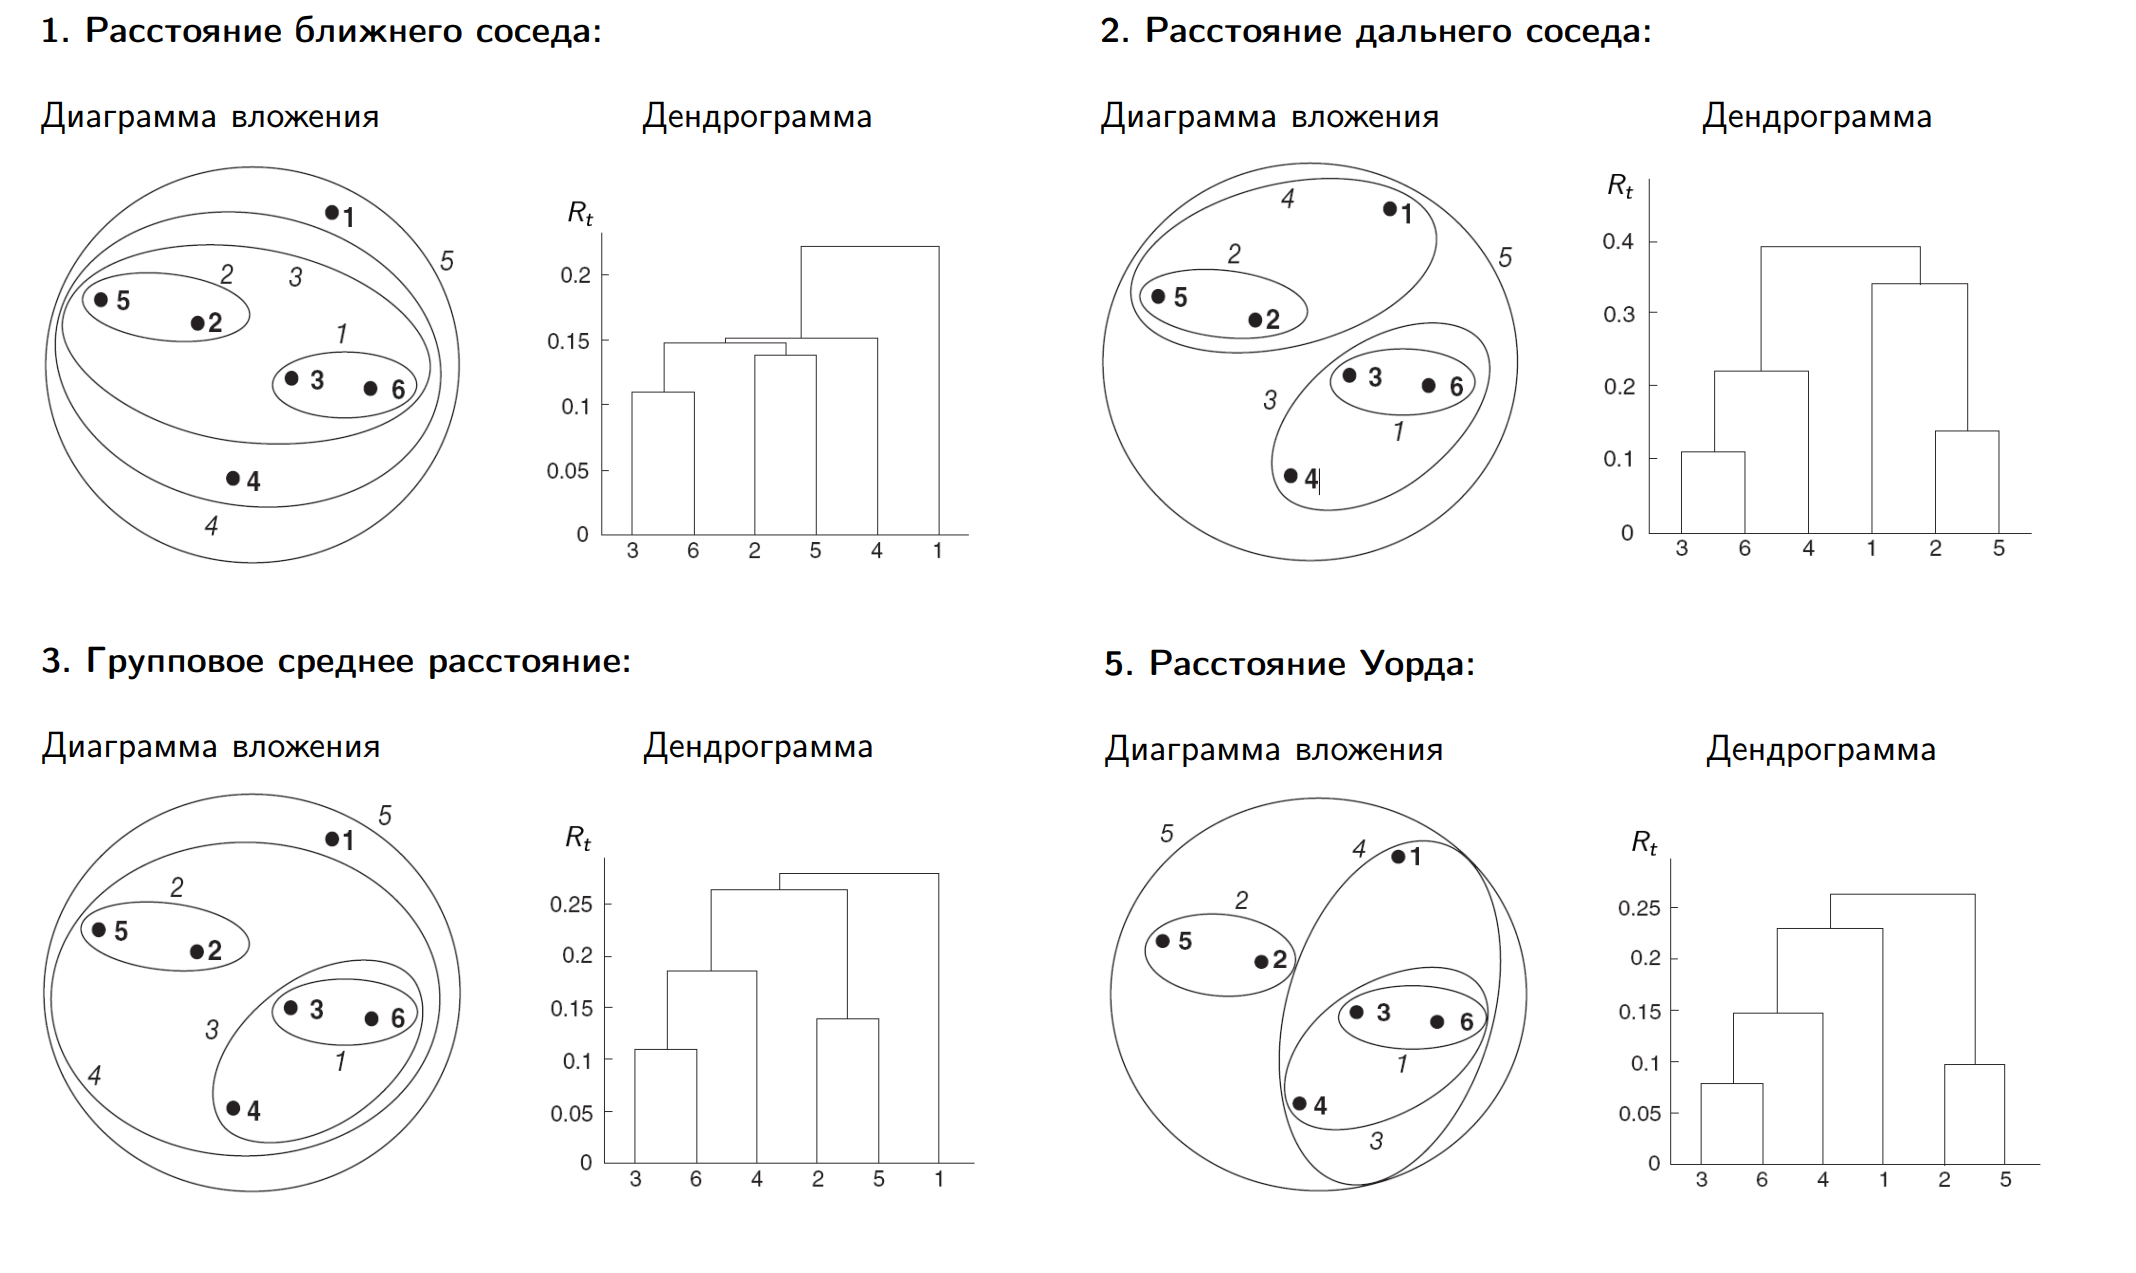
\includegraphics[scale=0.2]{hier.png}
	\caption{Дендрограммы при выборе различных расстояний.}
\end{figure}

Вторым желательным свойством является свойство растяжения. Кластеризация называется сжимающей, если $R_t \leq \rho(\mu_U, \mu_V), \forall t$ и называется растягивающей, 
если $R_t \geq \rho(\mu_U, \mu_V), \forall t$.
При выборе сжимающих расстояний объекты с каждым шагом всё больше слипаются друг с другом.
Свойство растяжения же позволяет лучше отделять кластеры друг от друга. 
Однако, при этом расстояние не должно быть сильно растягивающим, иначе объекты удалятся друг от друга настолько, что появится много лишних кластеров. 
В качестве меры растяжения рассматривается отношение расстояния между кластерами к расстоянию между центрами кластеров. 

Относительно приведённых свойств самыми оптимальными оказываются расстояние Уорда и гибкое расстояние, 
а расстояние между центрами оказывается самым плохим, поскольку оно единственное не является монотонным. 
При этом гибкое расстояние оказывается сжимающим при $\beta >0$ и растягивающим при $\beta <0$. 

Существует также редуктивная версия алгоритма, для которой требуется выполнения свойства редуктивности. 
Отметим, что из представленных расстояний только расстояние между центрами не является редуктивным.

Одним из достоинств иерархической кластеризации является получение в результате дендрограммы, которая может представлять самостоятельный интерес. 

\section{Функционалы качества}

В задаче кластеризации без модели отсутствует естественный функционал качества. Однако, его можно ввести в рассмотрение самостоятельно. 
Тогда задача кластеризации уже ставится как задача максимизации или минимизации выбранного функционала.
Исходя из начальной постановки задачи <<меньше расстояние внутри кластеров --- больше снаружи>>, естественно выбрать среднее внутрикластерное расстояние 
$$F_0=\frac{\sum_{i<j} [y_i=y_j] \rho(x_i, x_j)}{\sum_{i<j} [y_i=y_j]}$$
или среднее межкластерное расстояние 
$$F_1=\frac{\sum_{i<j} [y_i \neq y_j] \rho(x_i, x_j)}{\sum_{i<j} [y_i \neq y_j]}$$
в качестве функционалов. 
Можно также выбрать для минимизации отношение двух этих функционалов, и, таким образом, объединить оптимизируемые свойства. 

Существует ещё множество различных более сложных функционалов качества. К подобным относятся Силуэт и индекса Данна. 
Смысл всех таких функционалов один и тот же: попытаться описать близость в кластерах и дальность между ними. Силуэт кластеризации строится следующим образом.
Определяется принадлежность объекта своему кластеру как среднее расстояние от выбранного объекта до всех остальных объектов в его кластере 
$$c(x_i) = \frac{1}{|K_i| - 1} \sum_{x_j \in K_i, i \neq j} \rho(x_i, x_j)$$
и определяется принадлежность объекта другому кластеру, как среднее расстояние до всех объектов ближайшего чужого кластера 
$$b(x_i) = \min_{l \neq i} \frac{1}{|K_l|} \sum_{x_j \in K_l} \rho(x_i, x_l).$$

Cилуэт такого объекта тогда равен 
$$s(x_i) = \frac{b(x_i) - c(x_i)}{\max \{ c(x_i), b(x_i) \}},$$ 
если $|K_i| > 1$ и $s(x_i) =0 $, если $|K_i|=1.$

Естественным образом силуэт кластеризации определяется как среднее силуэтов всех объектов $S = \frac{1}{m} \sum_{i=1}^m s(x_i)$.

Значения силуэта изменяются от $-1$ до $+1$, и кластеризация удалась лучше, если значение силуэта больше. Значения силуэта можно интерпретировать так: $-1$ --- кластеризация
точно не удалась, $0$ --- удалась кластеризация или нет относительно силуэта неизвестно, $+1$ --- кластеризация точно удалась. Обычно, желательно, чтобы значение силуэта
для кластеризации оказалось не менее $0.75$.

Как видно из определения, для вычисления силуэта необходимо, чтобы кластеров было как минимум два. Ещё одна проблема его в том, 
что он не очень корректно обрабатывает ленточные кластеры, перекрывающиеся и кластеры с перемычками. Как только расстояние между объектами одного кластера становится 
сравнимым с расстоянием между объектами разных кластеров, силуэт перестаёт быть адекватным функционалом качества.
Кроме того, в силуэт никак не заложен шум. Это значит, что если в данных встретится аутлаер, то силуэт будет больше (а значит, согласно ему, кластеризация удалась лучше), 
если аутлаер будет посчитан как отдельный кластер.

Таким образом, данный функционал качества заточен именно под кластеры такого вида, когда они представляют собой далеко отстоящие компактные скопления объектов.

Индекс Данна 
$$D = \frac{\min_{1 \leq i < j < k} \delta(K_i, K_j)}{\max_{1 \leq s \leq k} \Delta(K_s)},$$
	где $\delta(K_i, K_j)$ --- расстояние между кластерами, $\Delta(K_s)$ --- диаметр кластера.

Для данного функционала качества характерны те же проблемы, что и для силуэта, только в ещё больших масштабах, 
поскольку в силуэте бралось усреднение расстояний между объектами, а в индексе Данна берутся минимальное между кластерами и максимальное внутри кластера расстояния.

Существует ещё группа функционалов, которая использует внешнюю информацию об априорном разделении объектов на кластеры. 
К таковым относятся, например, Rand Index, Jaccard Index, Minkowski Score.
Однако, подобные задачи уже не являются задачами обучения без учителя.

\section{Другие эвристические алгоритмы}

\subsection{FOREL}
Рассмотрим ещё несколько эвристических алгоритмов. Алгоритм FOREL предложен Загоруйко и Ёлкиной в 1967 году
при решении одной прикладной задачи в области палеонтологии. Алгоритм имеет
многочисленные вариации. В основе всех этих вариаций лежит следующая базовая процедура.

Берётся некоторый объект из выборки $x_0 \in X^m$ и параметр $R$. Выделяются все объекты выборки $x_i \in X^m$, попадающие внутрь сферы $\rho(x_i, x0) < R$, 
и точка $x_0$ переносится в центр тяжести выделенных точек. Эта процедура повторяется до тех пор, пока
состав выделенных точек, а значит и положение центра, не перестанет меняться.
Доказано, что эта процедура сходится за конечное число шагов. Центр сферы $x_0$ в общем случае
не является объектом выборки, потому и называется формальным элементом.

Алгоритм FOREL:
	\begin{enumerate}
	\item Пусть $U=X^m$
	\item \textbf{Пока} есть некластеризованные точки, т.е. $U \neq \varnothing$;
	\item \quad взять случайную точку $x_0 \in U$;
	\item \quad \textbf{Повторять}
	\item \qquad образовать кластер с центром в $x_0$ и радиусом $R$:

		\qquad $K_0 = \{ x_i \in U ~|~ \rho(x_i, x_0) \leq R \};$
	\item \qquad переместить центр $x_0$ в центр масс кластера:

		\qquad $x_0 = \frac{1}{|K_0|} \sum_{x_i \in K_0} x_i;$
	\item \quad \textbf{Пока} состав кластера $K_0$ не стабилизируется;
	\item \quad $U= U \setminus K_0;$
	\item применить алгоритм КНП к множеству центров кластеров;
	\item каждый $x_i \in X^m$ приписать кластеру с ближайшим центром;
	\end{enumerate}

Алгоритм кратчайшего незамкнутого пути (КНП):
	\begin{enumerate}
	\item Найти пару вершин $(x_i, x_j) \in X^m$ с наименьшим $\rho(x_i, x_j)$ и соединить их ребром;
	\item \textbf{Пока} в выборке остаются изолированные точки
	\item \quad найти изолированную точку, ближайшую к 

		\quad некоторой неизолированной;
	\item \quad соединить эти две точки ребром;
	\item удалить $k-1$ самых длинных рёбер;
	\end{enumerate}

Если присмотреться внимательно к алгоритму, то можно узнать в нём k-means, только теперь радиус сфер берётся в качестве параметра. 
Кроме того, в FOREL присутствует объедиенение полученных сфер каким-либо алгоритмом в кластеры побольше, уже не обязательно сферические 
(в алгоритме выше был предложен для этих целей алгоритм КНП, но можно взять и другой).

\subsection{DBSCAN}
DBSCAN --- это эвристический алгоритм кластеризации, который предложили Маритин Эстер, Ганс-Петер Кригель, Ёрг Сандер и Сяовэй Су в 1996. 
Это алгоритм кластеризации, основанный на плотности --- алгоритм группирует вместе те объекты, которые тесно расположены, 
помечая как выбросы объекты, которые находятся в областях с малой плотностью. 

	В этом алгоритме рассматривается для каждого объекта $x \in U$ его $\eps$-окрестность $U_\eps (x) = \{u \in U : \rho(x ,u ) \leq \eps\}$.
	Каждый объект может быть одного из трёх типов:
	\begin{itemize}
	\item корневой: имеет плотную окрестность $|U_\eps (x)| \geq m$
	\item граничный: не корневой, но находится в окрестности корневого
	\item выброс: не корневой и не граничный.
	\end{itemize}
Корневые объекты находящиеся в $\eps$-окрестности друг друга объединяются в один кластер. Граничные объекты относятся к тому кластеру, к какому относится корневой
объект, в $\eps$-окрестности которого лежит данный граничный объект. Таким образом, в итоге получается разделение всех объектов на кластеры и шумовые объекты.
Более подробный алгоритм приведён ниже.
	\begin{enumerate}
		\item $U=X^m$, $N=\varnothing$, $z=0$;
		\item \textbf{Пока} есть некластеризованные точки, т.е. $U \neq \varnothing$;
		\item \quad взять случайную точку $x \in U$;
		\item \quad \textbf{если} $|U_\eps (x)| < m$, \textbf{то}
		\item \qquad пометить $x$ как шумовой;
		\item \quad \textbf{иначе}
		\item  \qquad создать новый кластер: $K=U_\eps (x)$; $z = z + 1$;
		\item \qquad \textbf{для всех} $x' \in K$
		\item \hskip 3em \textbf{если} $|U_\eps (x')| \geq m$ \textbf{то} $K=K \cup U_\eps(x')$;
		\item \hskip 3em \textbf{иначе} пометить $x'$ как граничный элемент $K$;
		\item \qquad $a(x_i) = z$ для всех $x' \in K$;
		\item \qquad $U=U \setminus K$;
	\end{enumerate}



	\begin{figure}[h]
	\centering
		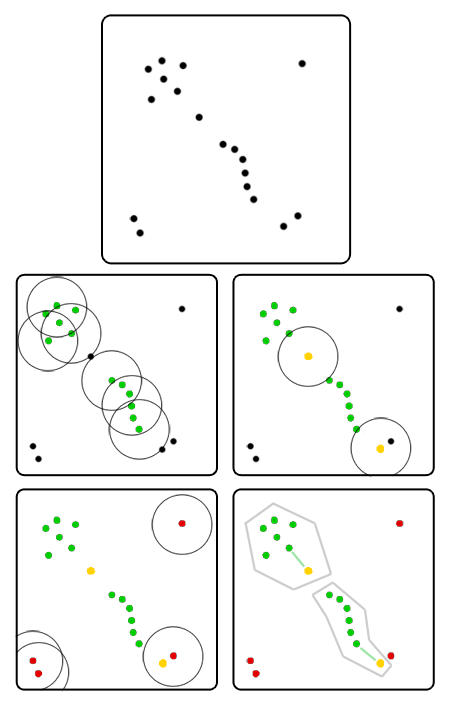
\includegraphics[scale=1.5]{dbscan.png}
	\caption{Иллюстрация к алгоритму DBSCAN. На рисунке зелёным отмечены корневые объекты, жёлтым --- граничные и красным --- шумовые.}
	\end{figure}



	\begin{figure}[h]
	\centering
		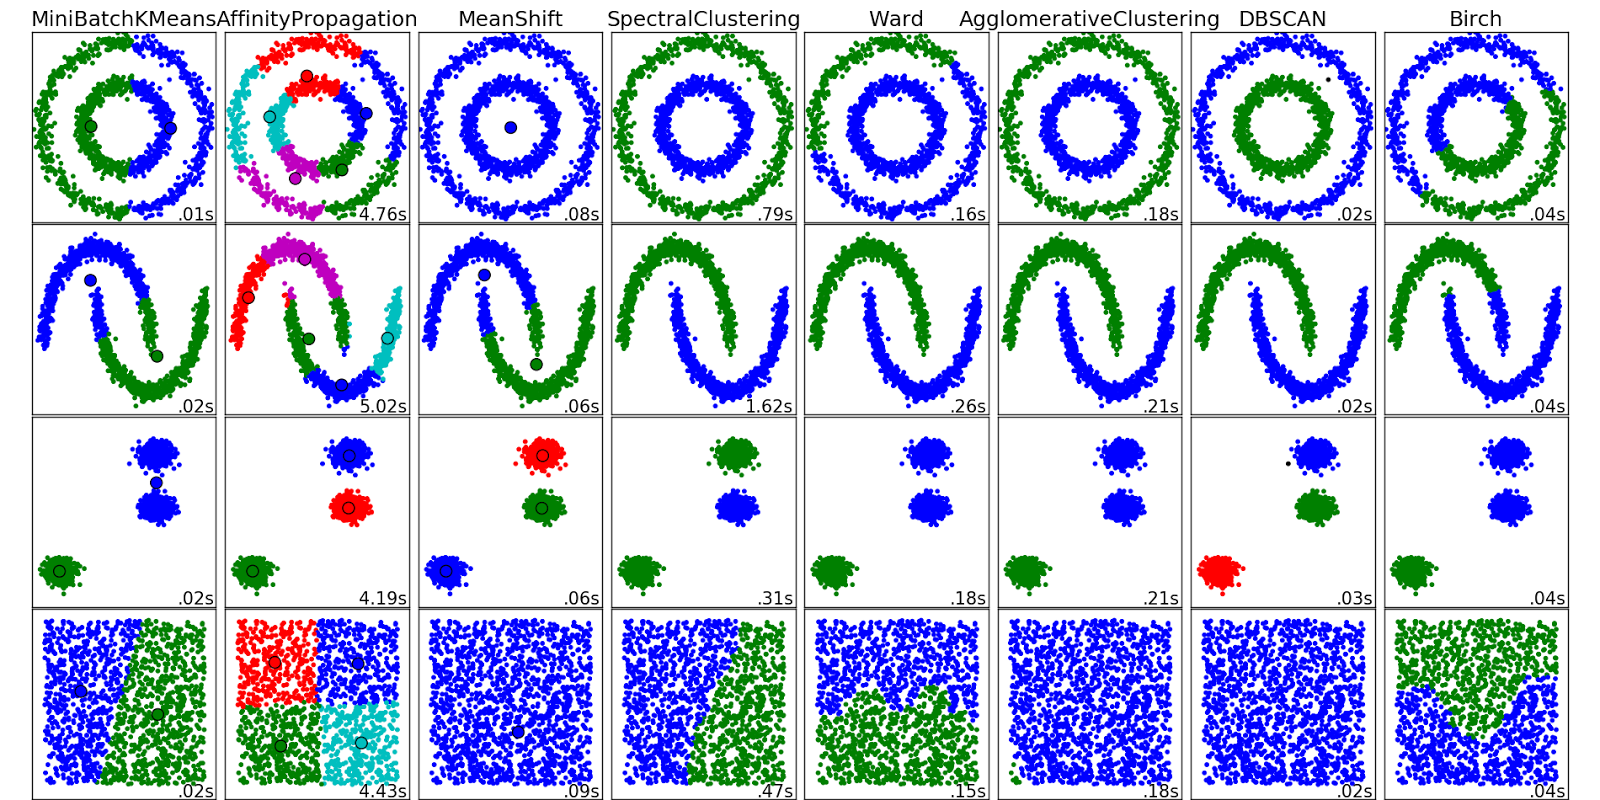
\includegraphics[scale=0.25]{dbscanexamp.png}
		\caption{Пример работы DBSCAN (второй столбец справа)}
		\label{fig:DBSCANres}
	\end{figure}

	Алгоритм DBSCAN считается довольно быстрым (от $O(m \ln m)$ до $O(m^2)$ в зависимости от реализации) и позволяет обрабатывать кластеры произвольной формы 
	(см.~рис.~\ref{fig:DBSCANres}).
	Помимо этого, DBSCAN выдаёт помимо деления на кластеры ещё и разметку шумовых объектов. Алгоритм хорошо поддаётся модифицированию 
	(существуют реализации, скрещенные с k-means и даже с GMM).
	
	Однако DBSCAN может плохо обрабатывать данные, в которых есть сильные вариации плотности внутри кластера, проёмы и шумовые мосты между кластерами.
\end{document}
